\chapter{Diagrammes Logiciel}
Les prochains diagrammes ont pour but de présenter notre architecture logicielle. Le diagramme de classes offre une vue d'ensemble sur les différentes composantes de la partie logicielle du projet. Les diagrammes de séquences montrent comment les différentes composantes interagissent entre elles. Les diagrammes de séquences sont divisés en plusieurs sous-tâches du défi afin d'améliorer la lisibilité.

\begin{landscape}
\begin{figure}
  \centering
  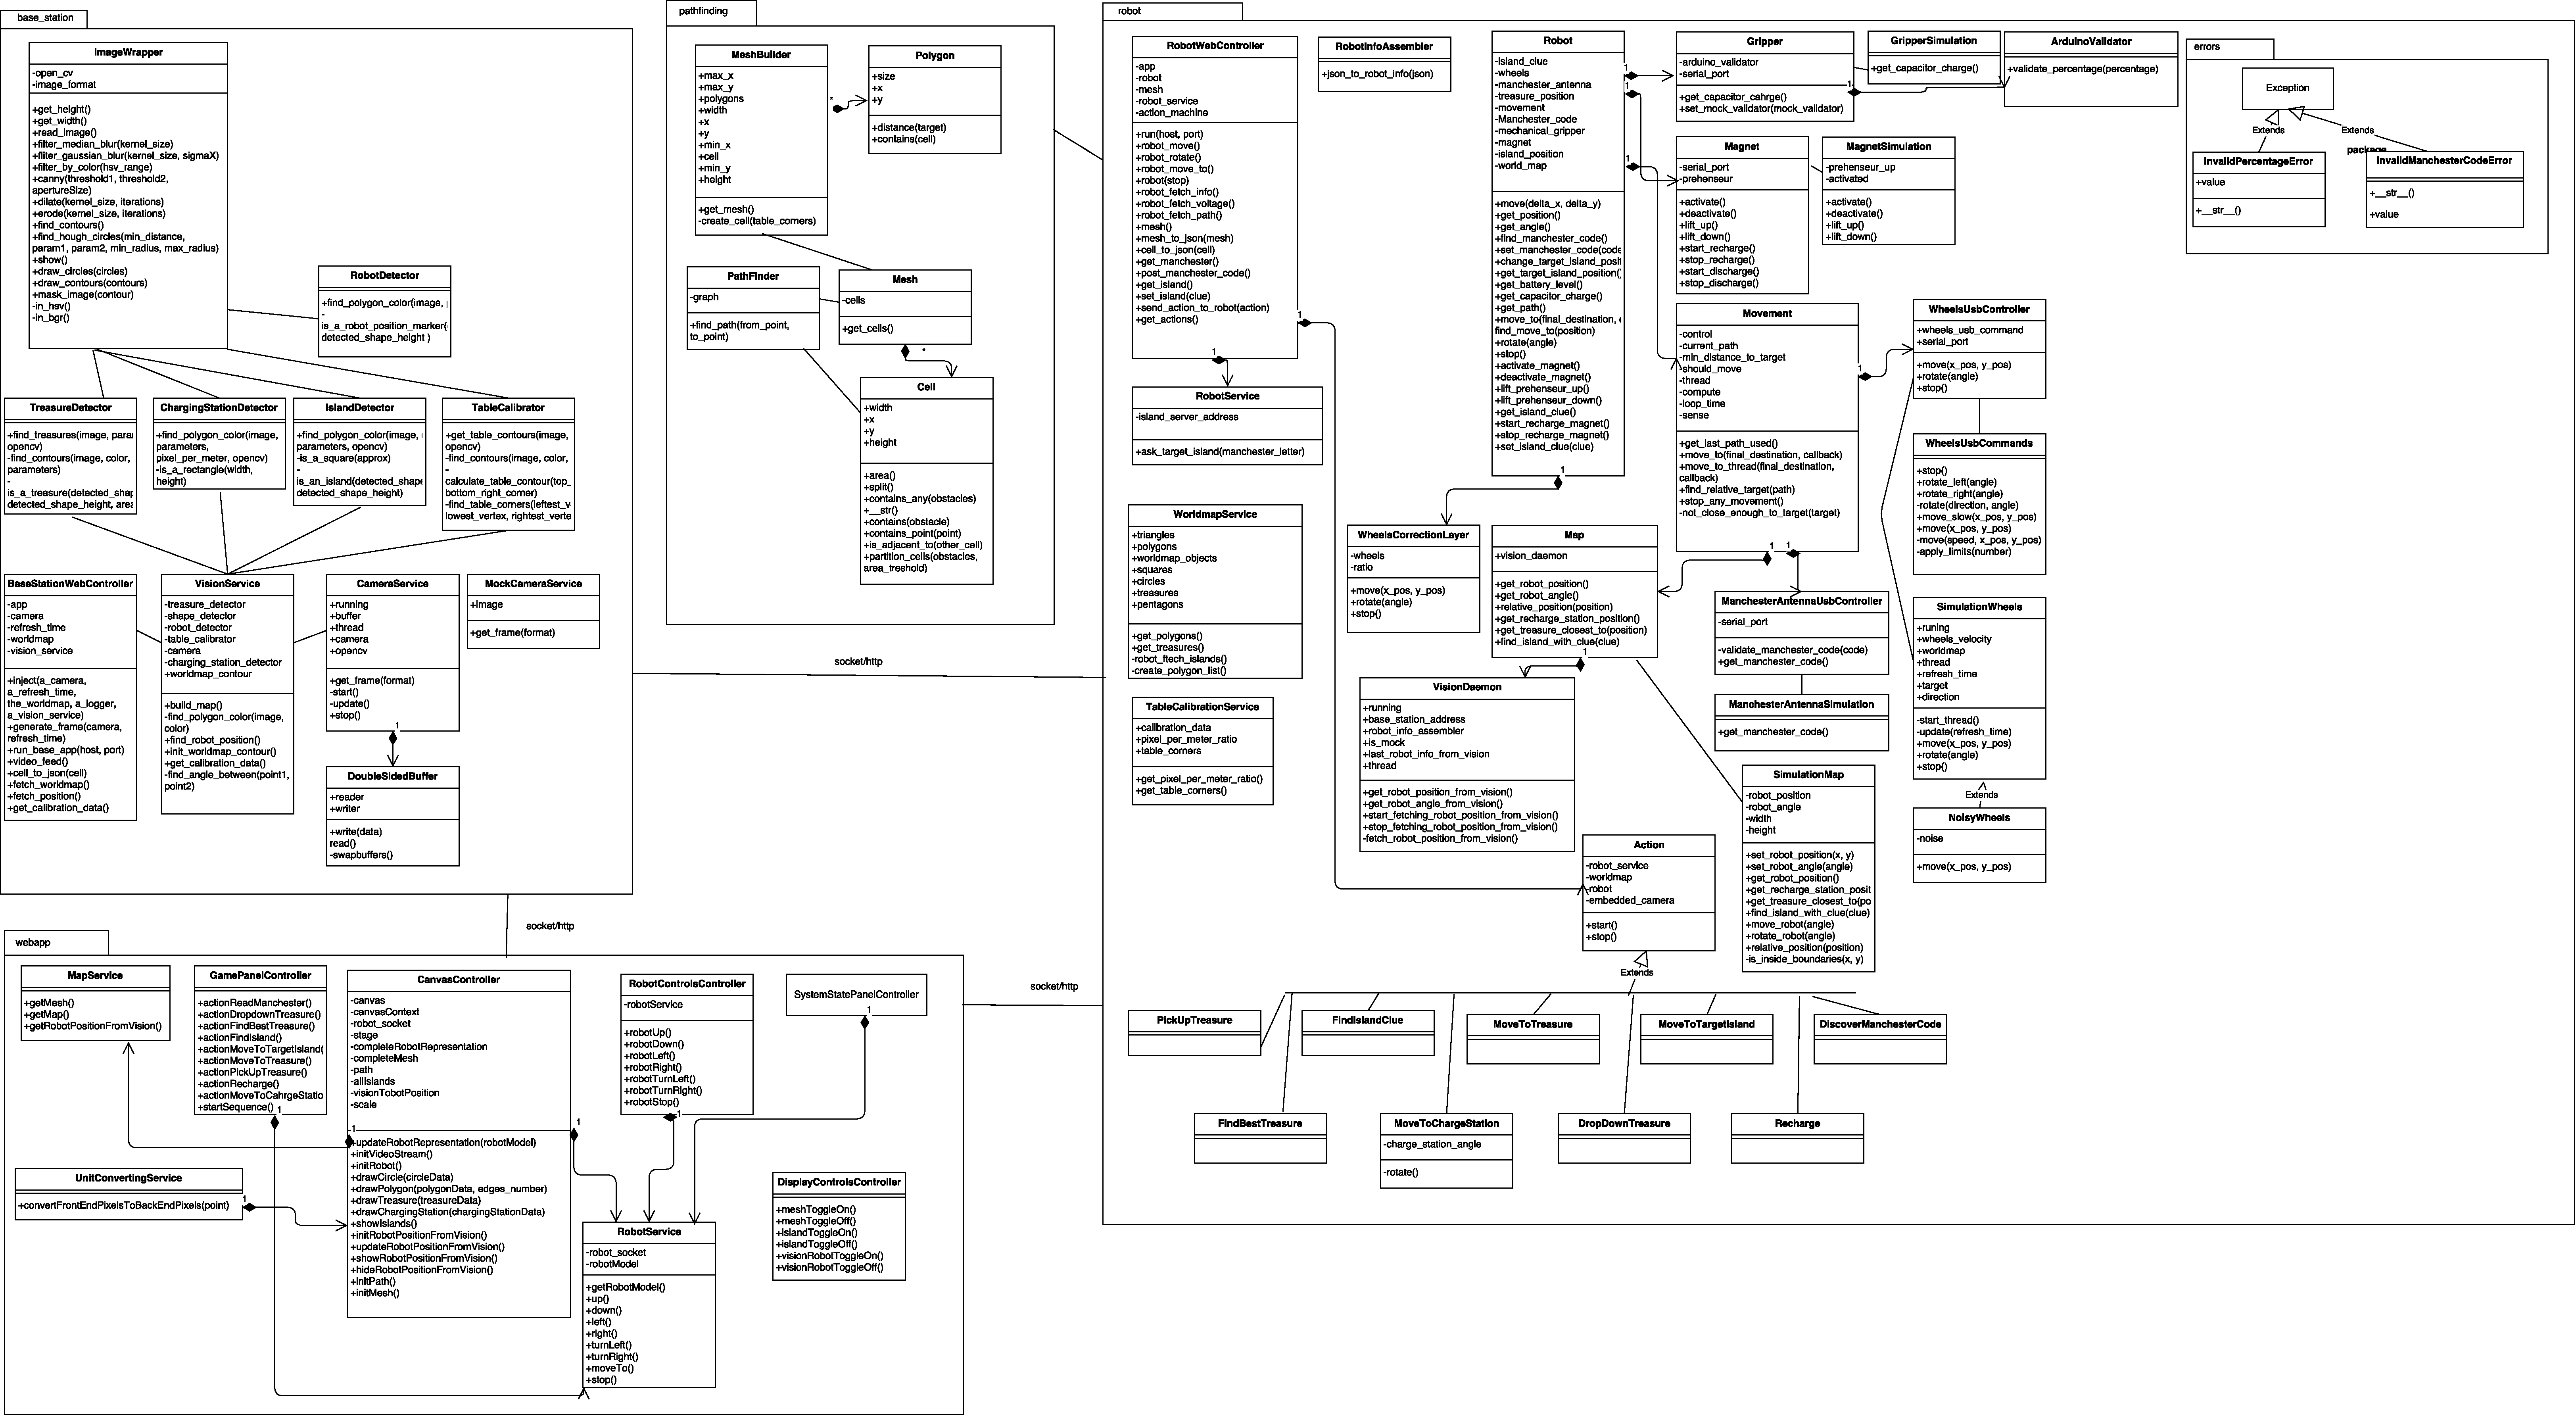
\includegraphics[scale=0.2, angle=0]{resources/diagrams/classDiagram.pdf}
  \caption{Diagramme de classes}
\end{figure}

\begin{figure}
  \centering
  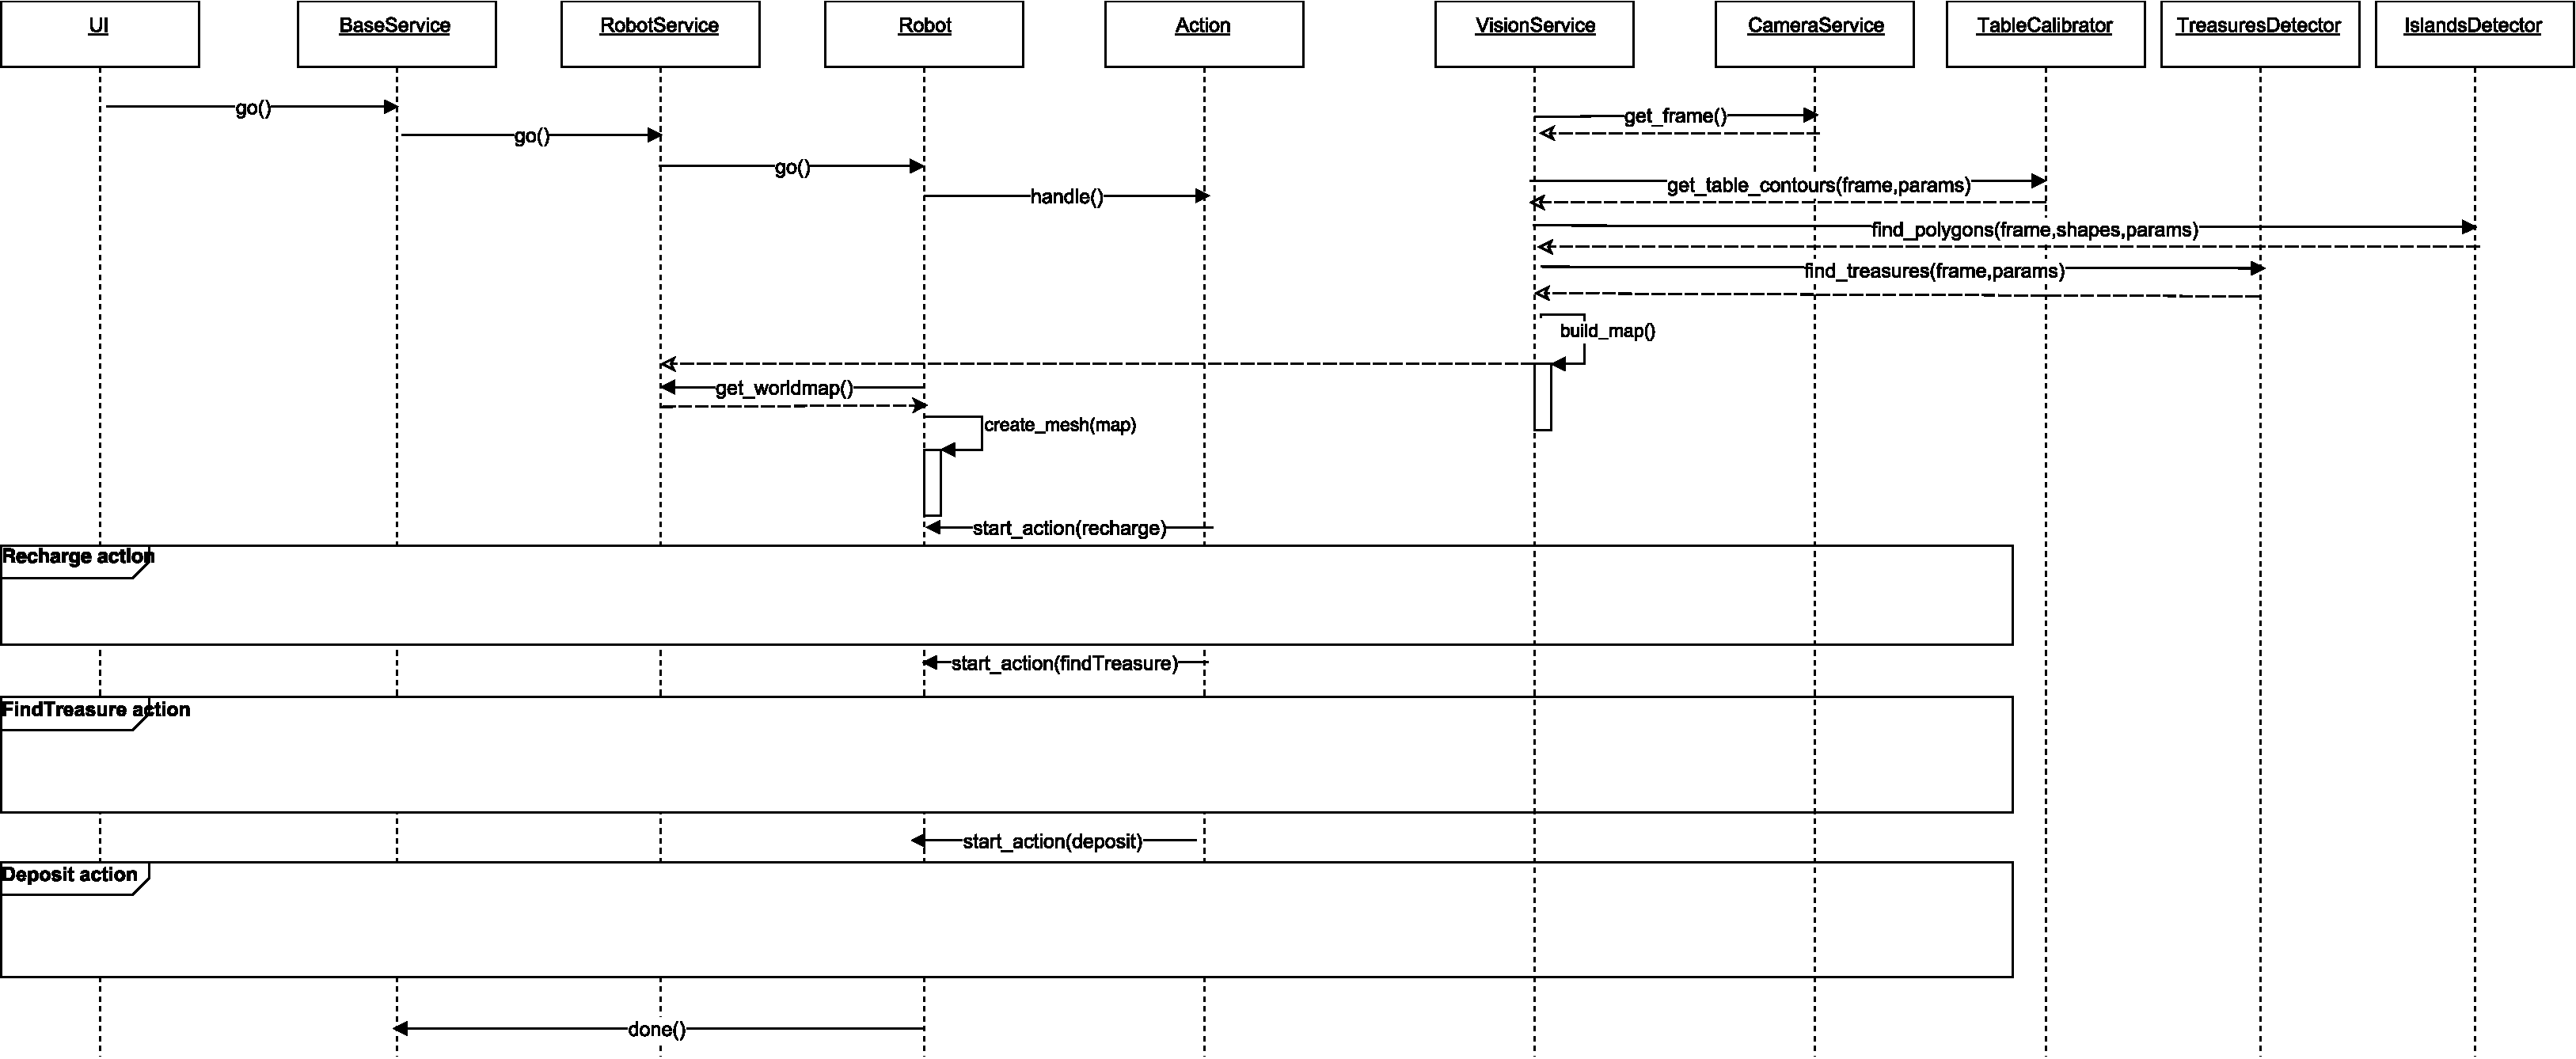
\includegraphics[scale=0.45, angle=0]{resources/diagrams/sequenceDiagram.pdf}
  \caption{Diagramme de séquence complet}
\end{figure}

\begin{figure}
  \centering
  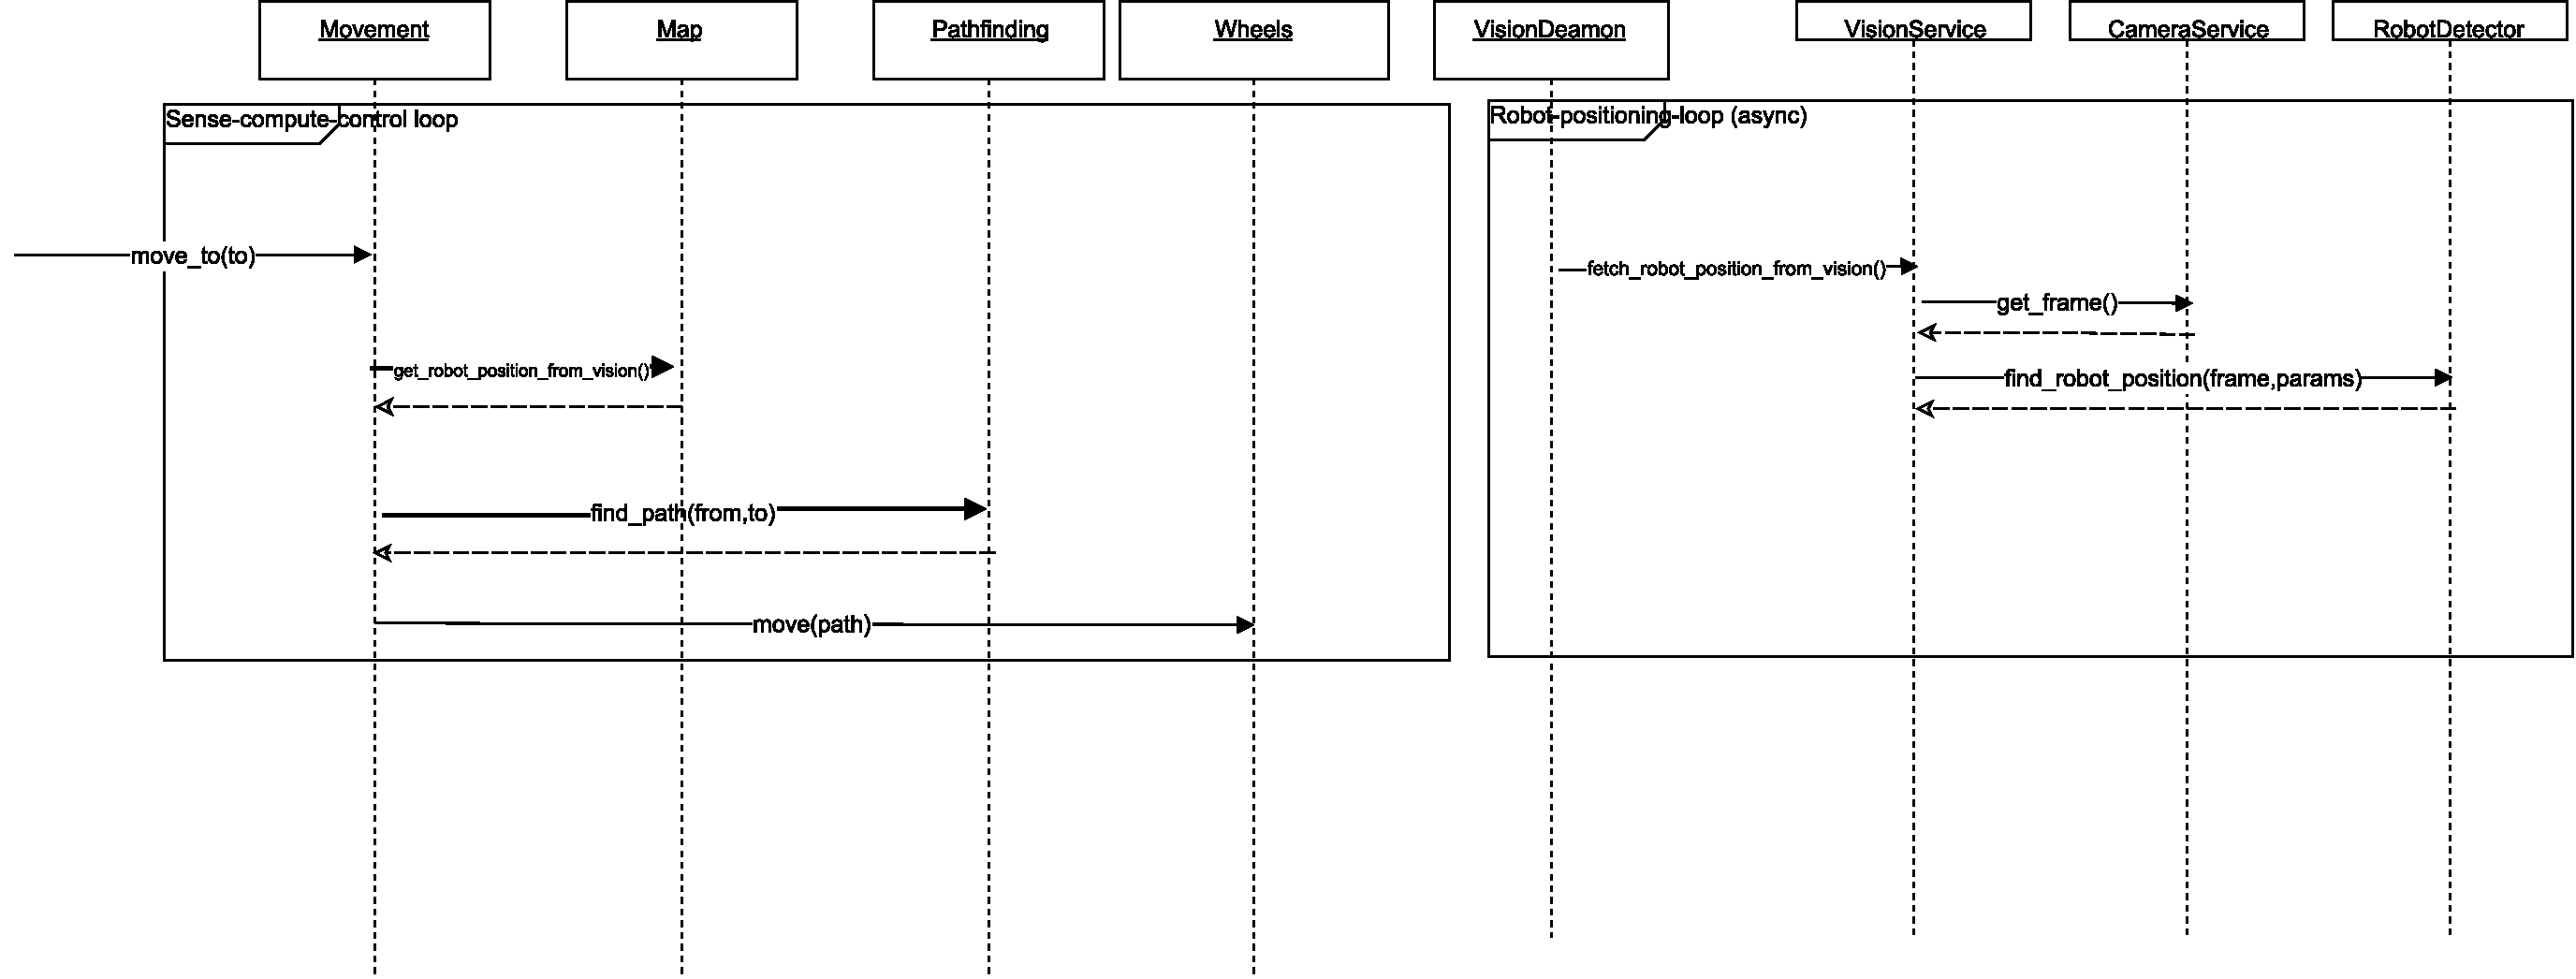
\includegraphics[scale=0.45, angle=0]{resources/diagrams/robotMovement.pdf}
  \caption{Diagramme de séquence de la boucle de sense-compute-control lors d'un déplacement}
\end{figure}

\begin{figure}
  \centering
  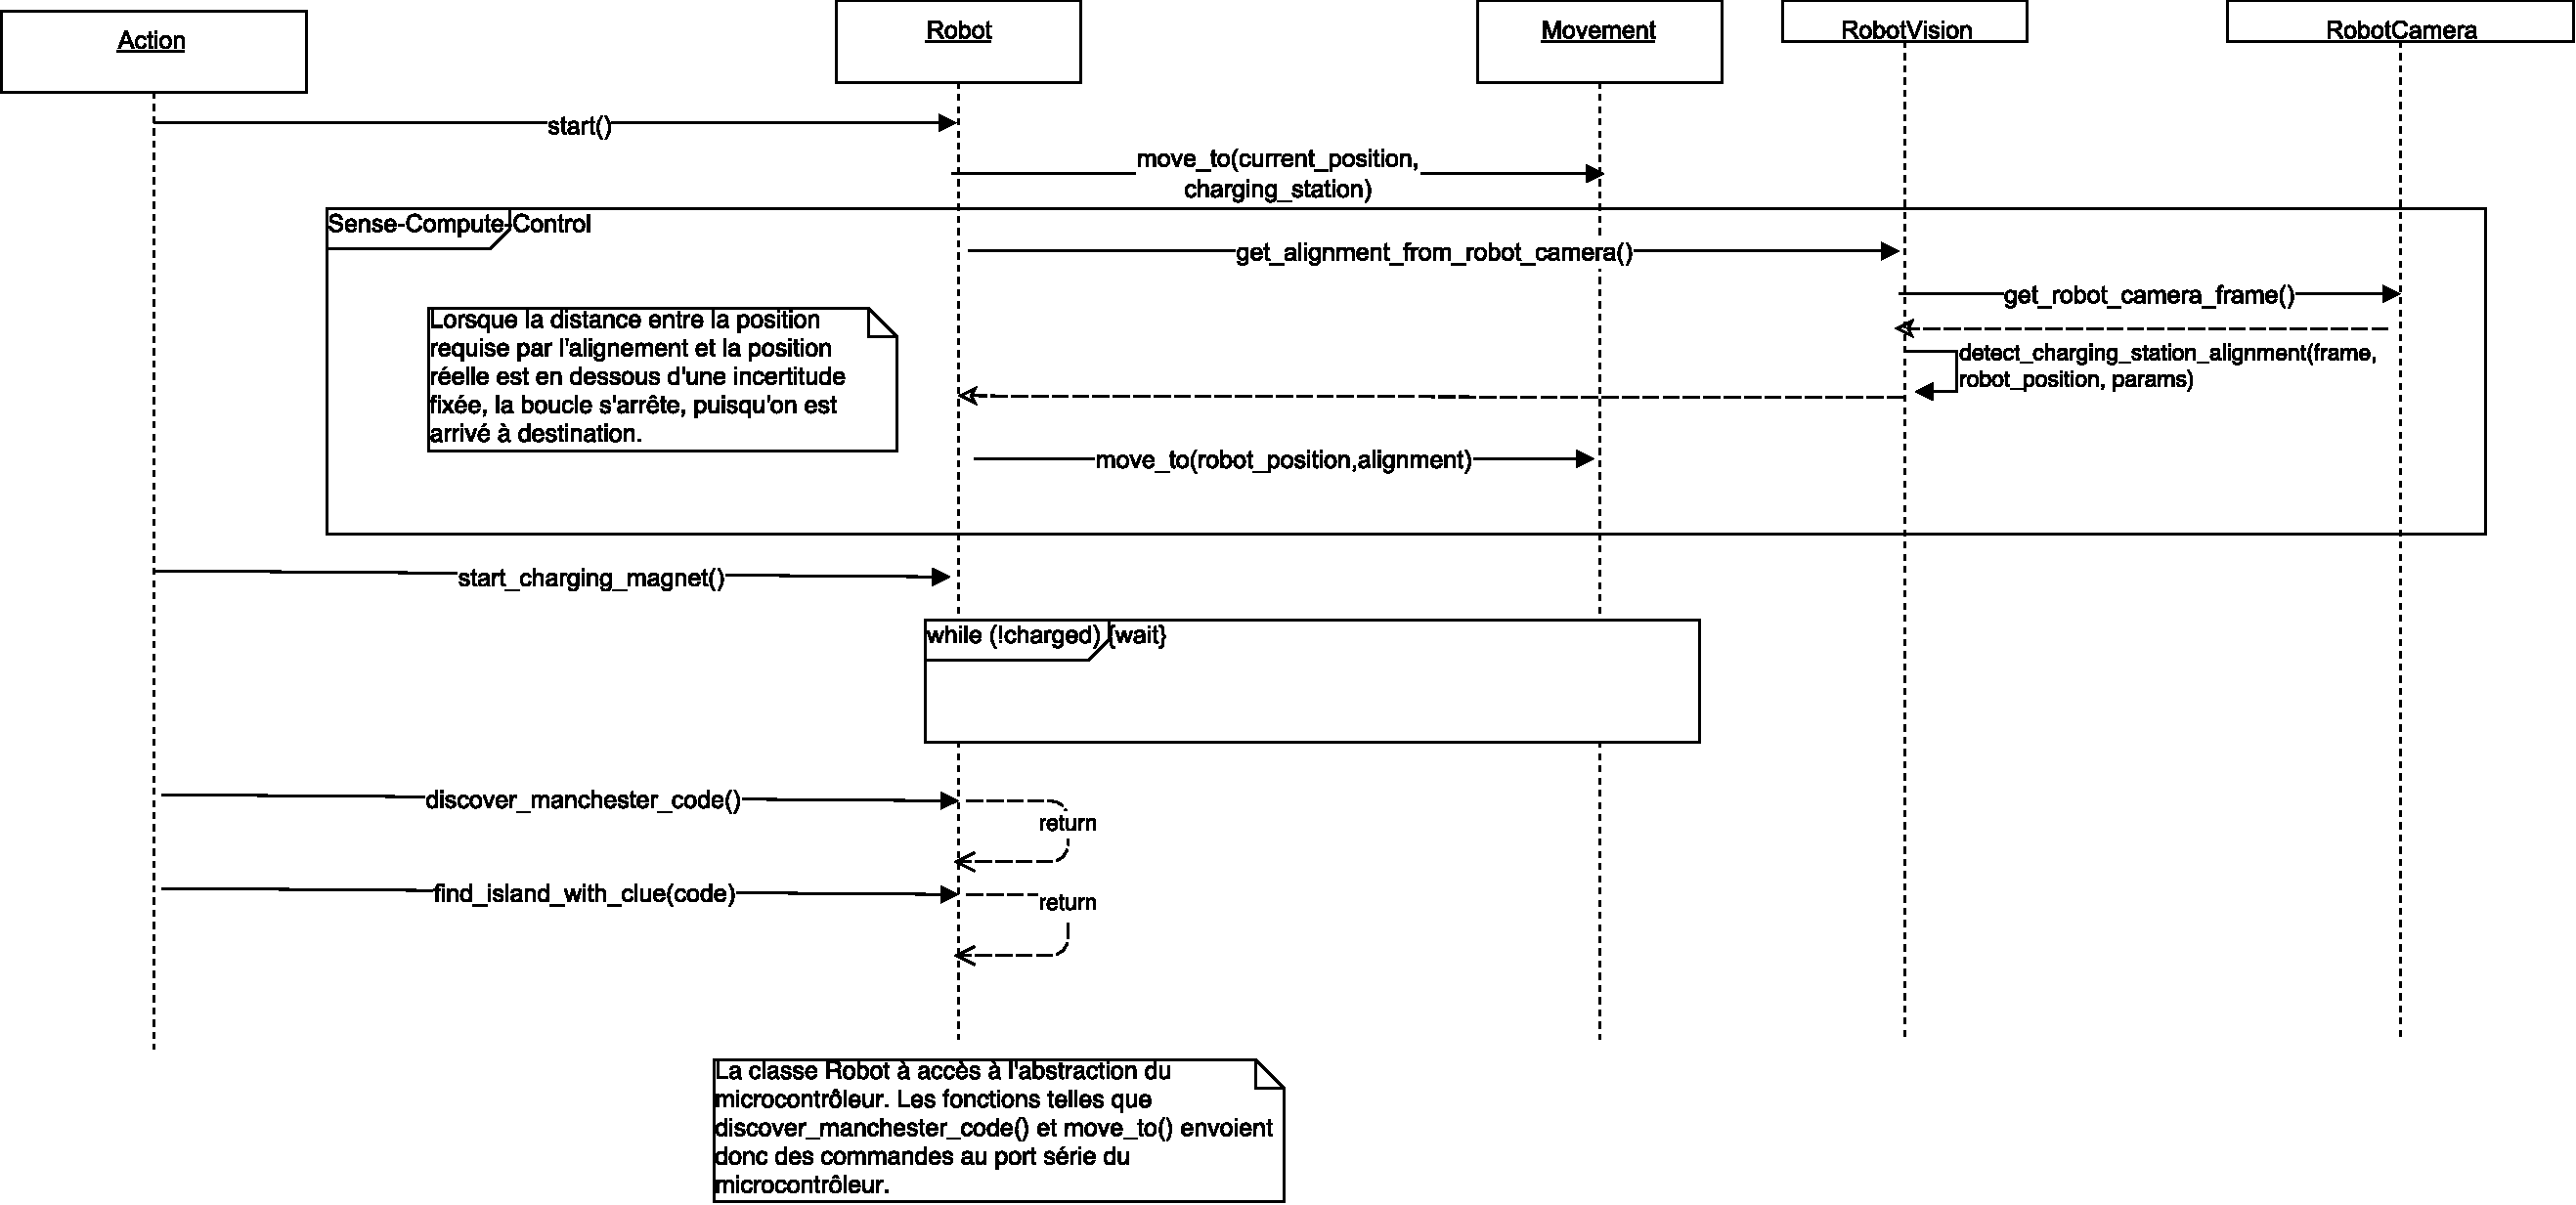
\includegraphics[scale=0.5, angle=0]{resources/diagrams/rechargeAction.pdf}
  \caption{Diagramme de séquence de recharge}
\end{figure}

\begin{figure}
  \centering
  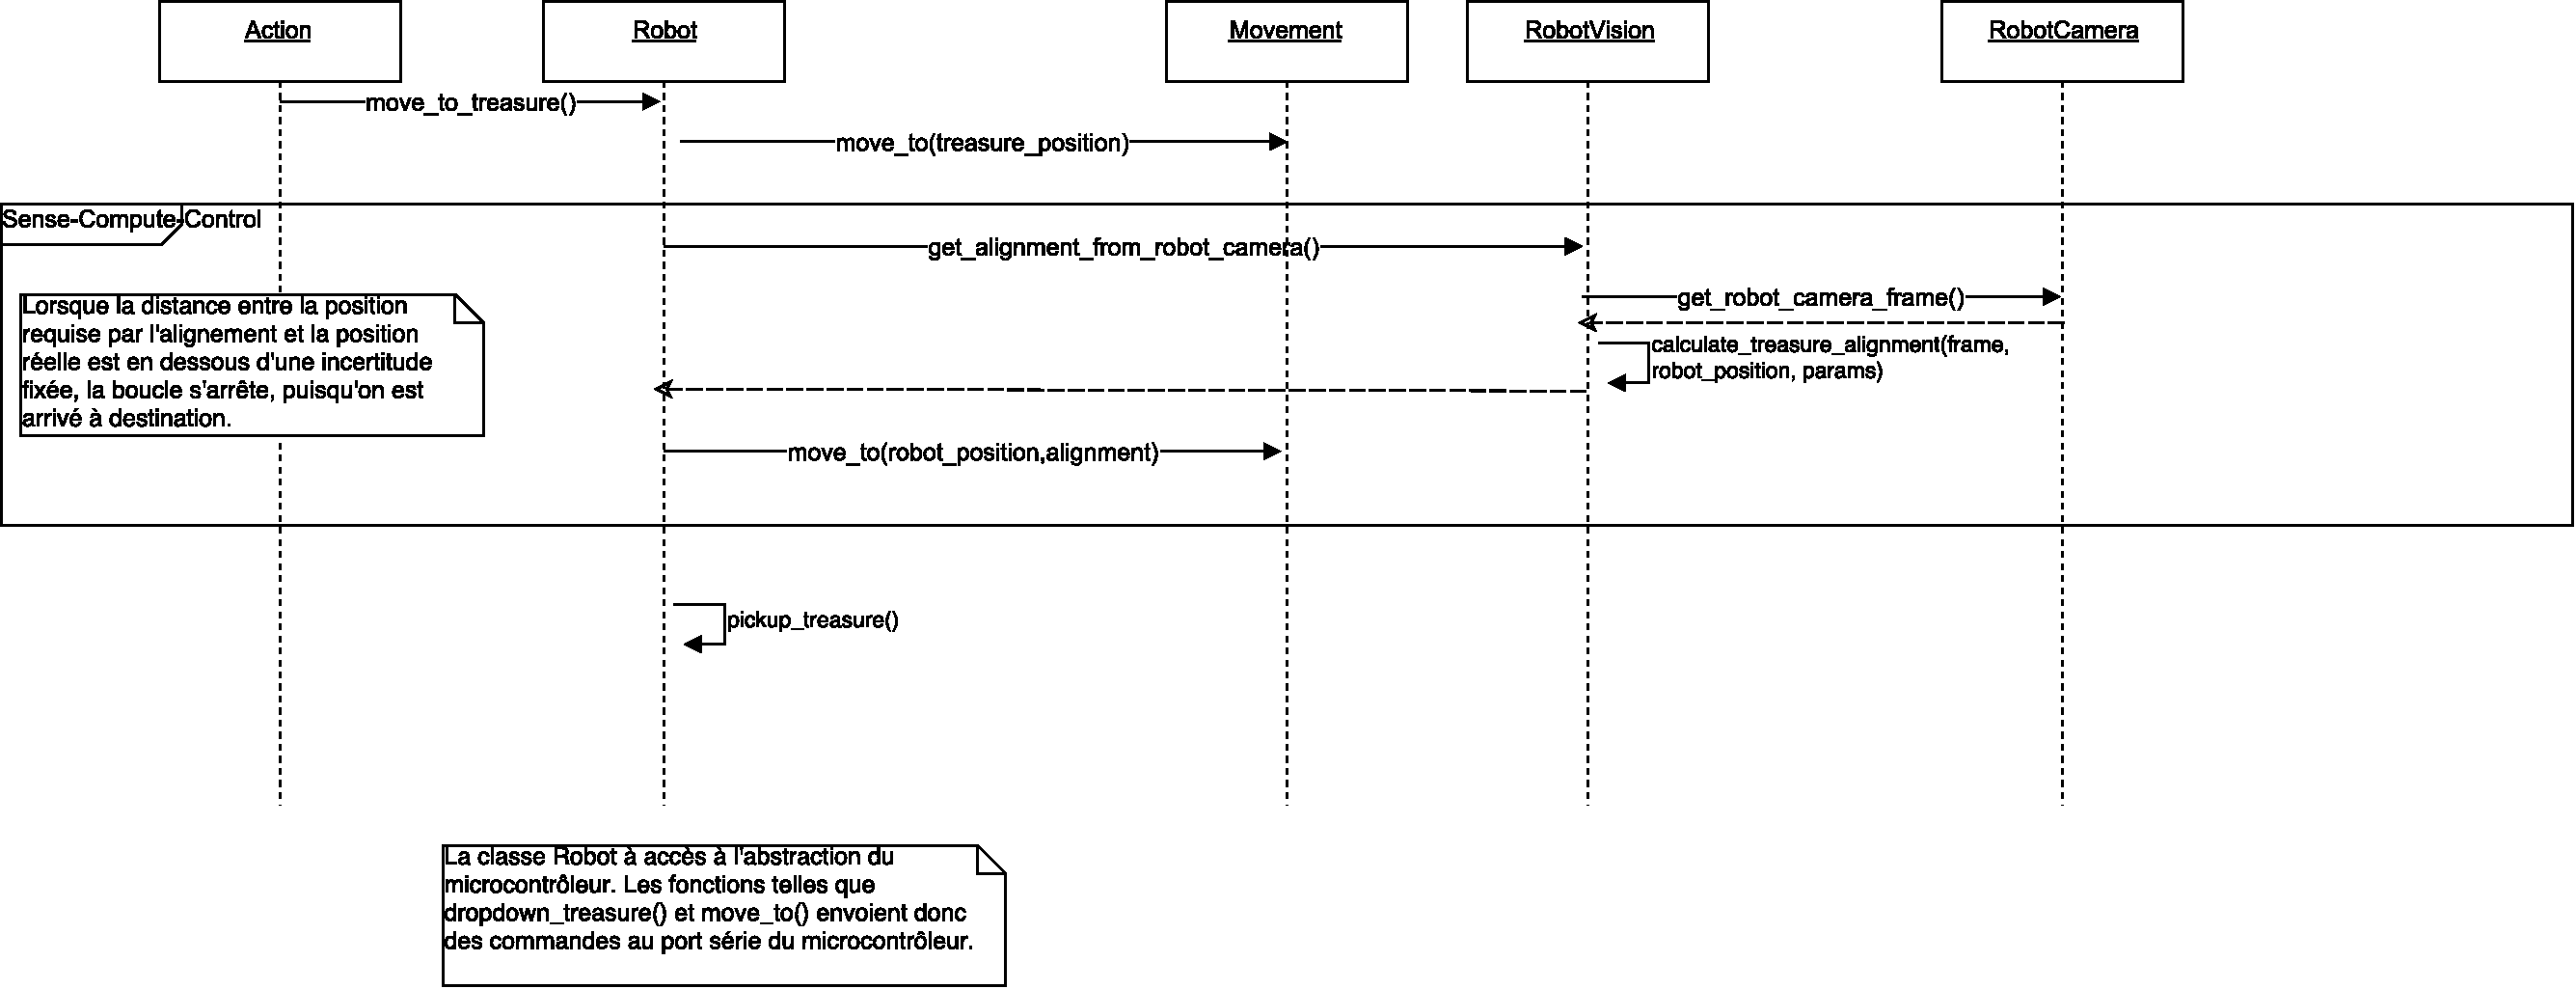
\includegraphics[scale=0.4, angle=0]{resources/diagrams/findTreasureAction.pdf}
  \caption{Diagramme de séquence de recherche de trésor}
\end{figure}

\begin{figure}
  \centering
  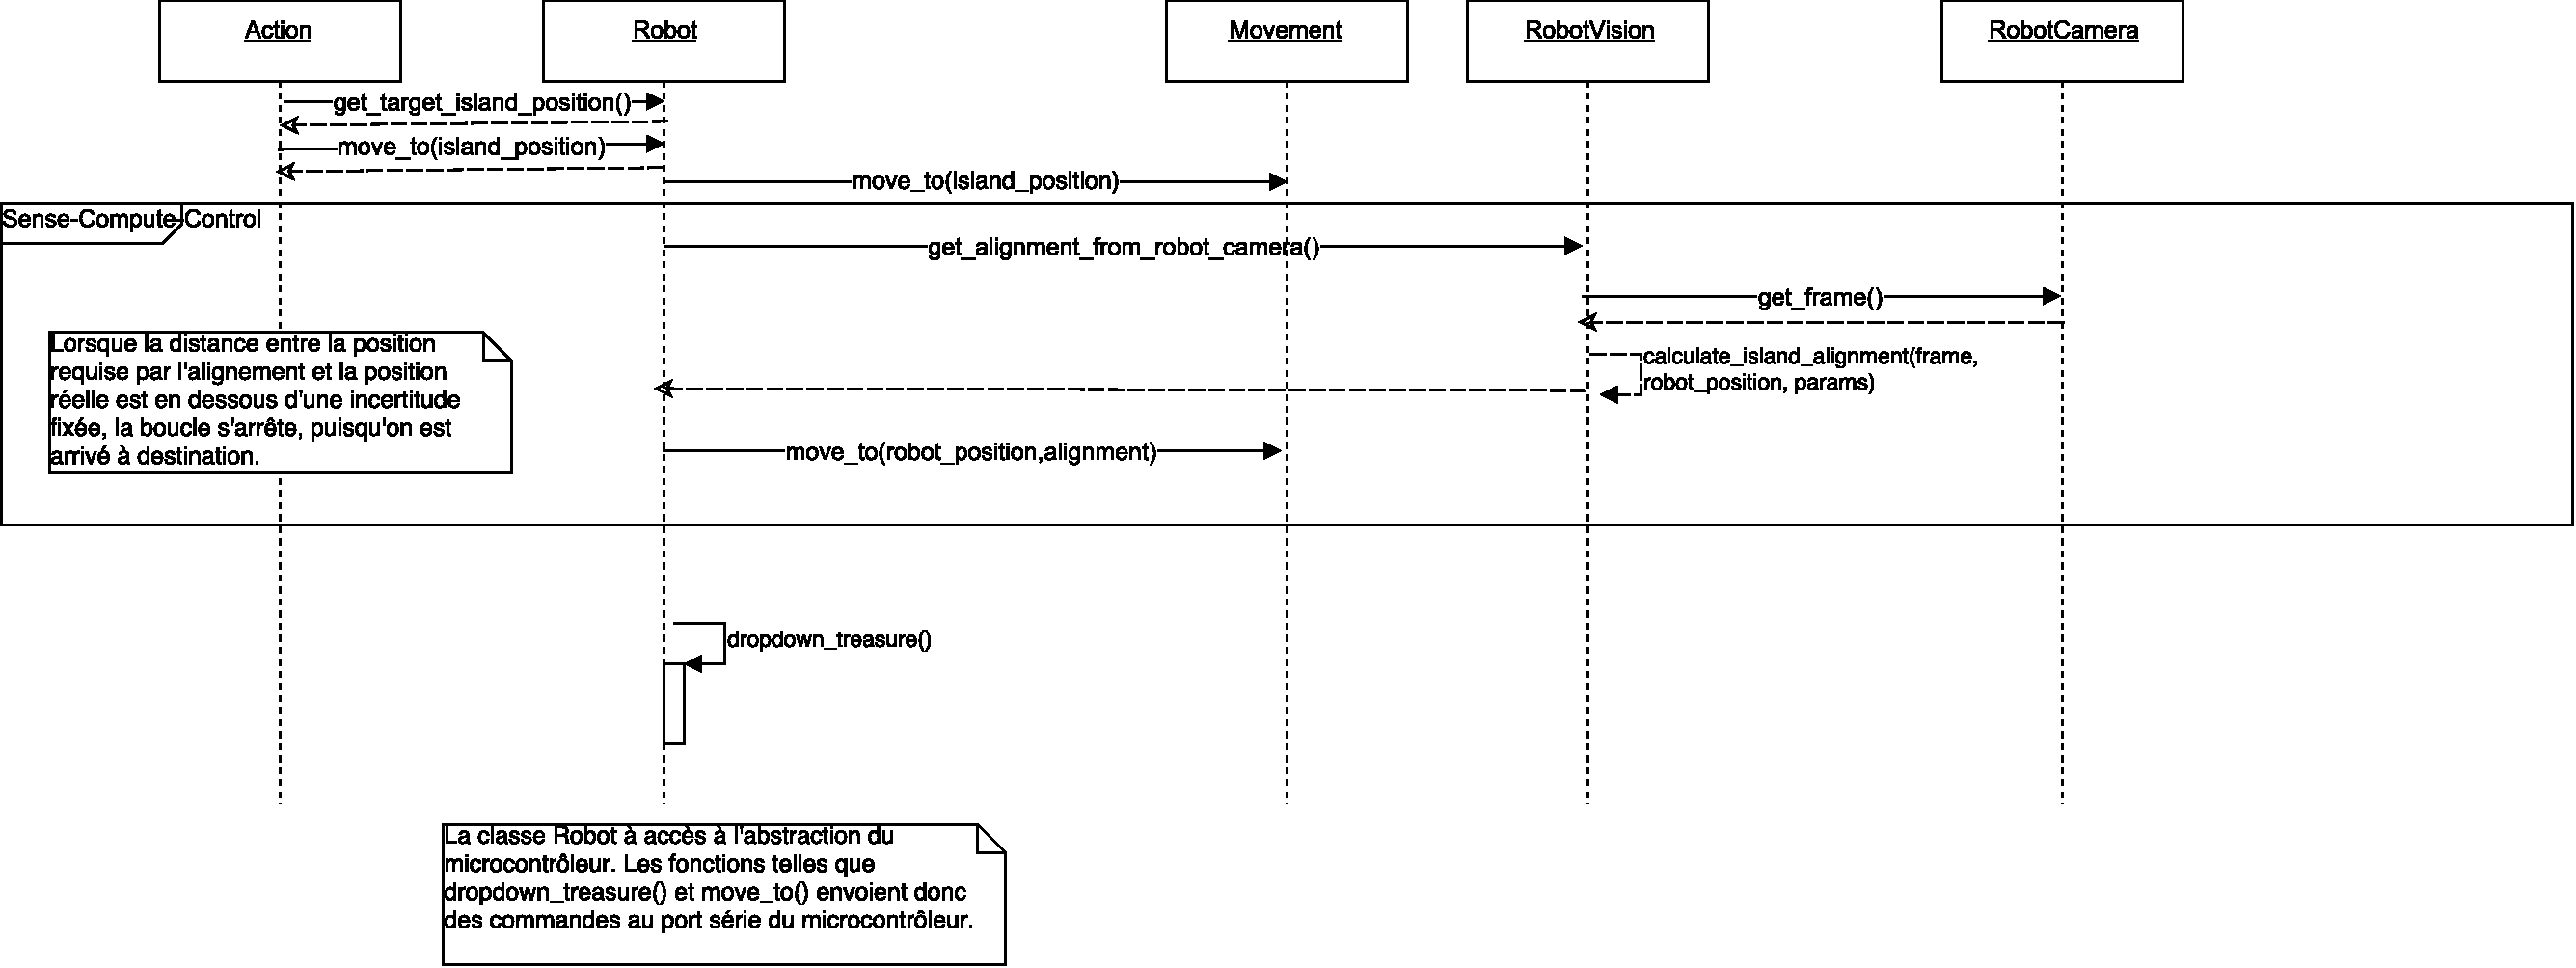
\includegraphics[scale=0.5, angle=0]{resources/diagrams/depositAction.pdf}
  \caption{Diagramme de séquence dépot du trésor}
\end{figure}
\end{landscape}
